% Dieser Artikel kann in ein paar Jahren weg, wenn sich keiner der Erstis mehr
% an Bologna/das Diplom erinnert ;-)
\section{Bachelor/Master}

\begin{multicols}{2}
\begin{quote}
	\textit{\foreignlanguage{english}{I accept chaos, I'm not sure whether it accepts me.}}
	
	\hfill--- Bob Dylan
\end{quote}
Im Zusammenhang mit dem Bologna-Prozess wurde in Deutschland das Diplomstudium abgeschafft.
Stattdessen wurde das zweistufige System von Bachelor und Master eingeführt.

\textbf{Wichtige Ziele der Deklaration:}
\begin{itemize}
	\item die Schaffung eines Systems leicht verständlicher und vergleichbarer Abschlüsse
	\item Förderung der Mobilität (Erasmus, Erasmus+)
	\item Förderung der europäischen Zusammenarbeit im Bereich der Qualitätssicherung
\end{itemize}

\subsection{Die Umsetzung}
Das damals neue System überforderte schnell Universitäten und Studierende.
Die alten Studiengänge wurden eben mal modularisiert, ans Ende jedes Moduls eine für die Endnote zählende Klausur gesetzt und man erhoffte sich, dass insgeheim alles so weiterginge wie bisher.
Elektronische Prüfungssysteme wie QISPOS machten das Chaos dann perfekt.

In Deutschland musste zunächst, um die Zweistufigkeit zu gewähren, das international renommierte Diplom abgeschafft werden.
In der Regel wurde das Grundstudium durch den Bachelor ersetzt und das Hauptstudium nun in den Master gezogen.

Man interpretierte in den Bachelor hinein, dass dieser ein berufsqualifizierender Abschluss sein müsse.
Ein wenig scheint dahinter der Gedanke zu stehen, man könne Geld sparen, wenn die Studierenden nicht mehr 5, sondern nur noch 3~Jahre studieren.
Das hat sich allerdings in der Praxis nicht bestätigt\dots

\subsection{Internationalisierung}
Im Positiven hat sich jedoch die hohe Anrechenbarkeit von international absolvierten Credits gezeigt.
Die Zweistufigkeit kann einen Wechsel nach dem Bachelor in einen anderen Master ermöglichen, was insbesondere bei Physik einen hohen Grad an Spezial-Mastern zulässt.
Es bleibt nur zu hoffen, dass auch in Zukunft hier genügend Masterplätze zur Verfügung stehen.

Insgesamt haben sich Studierende und Professoren inzwischen an die Änderungen gewöhnt und können ihnen auch positive Seiten abringen.
Es bleibt zu hoffen, dass die Diskussion weiterlebt.

\fibelsig{Connie, Simon}
\end{multicols}

\begin{center}
	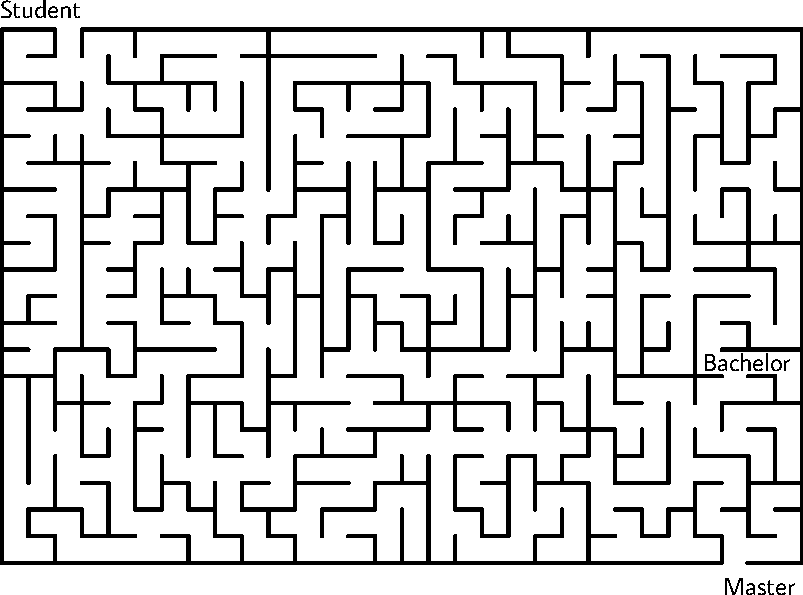
\includegraphics[width=\textwidth, height=0.38\textheight]{res/bachelor_master_labyrinth.pdf}
\end{center}
